\section{Вращающийся диполь}
Можем представить расположение одного из зарядов как:
\begin{eqnarray}
    x &=& r \cos \omega t\\
    y &=& r \sin \omega t
\end{eqnarray}

\begin{gather}
    d = e
    \begin{pmatrix}
        x \\ y
    \end{pmatrix}
    = e
    \begin{pmatrix}
        r\cos \omega t \\ r\sin \omega t
    \end{pmatrix}
    \implies 
    \ddot d =
    \begin{pmatrix}
        -r \omega \sin \omega t \\ r \omega \cos \omega t
    \end{pmatrix}
\end{gather}

Аналогично подставим в \ref{eq:J_ddotd}, получим:
\begin{eqnarray}
    \mathfrak{I} = \cfrac{\omega^2 r^2 e^2 }{8\pi c^3}(1 + \cos^2 \theta) do
\end{eqnarray}
Важно здесь угол $\theta$ это не тот угол $\phi$ что во 
второй части уравнения \ref{eq:J_ddotd}. $\phi$ это угол между $\ddot d$ и $n$, а $\theta$ 
это полярный угол.
Интегрирование по всем углам даст нам полное излеучение диполя 
\begin{equation}
    \mathfrak{I} = \cfrac{2e^2r^2w^2}{3c^3}
\end{equation}


Для определения поляризации вспомним \ref{eq:2.5}, нам важно только:
\begin{equation}
    H \sim \insqr{\ddot d, n}, \ \abs{H} \sim \sin \phi
\end{equation}
По картинке видно максимум $H$ выпадает на плоскость $n, z$ 
а минимум на поскость перпендикулярную ей и проходящюю через $n$. Таким 
образом $H_{max} \sim \ddot d$, $H_{min} \sim \ddot d \cos \theta$ от сюда 
отношение большей полуоси к меньшей $\cos \theta$, так же видно что поляризация 
элиптична. Но в если $n$ совпадает c $z$ то поряризация круговая, если 
$n$ лежит в $XY$ то поляризация линейная.


\begin{figure}[H]
    \centering
    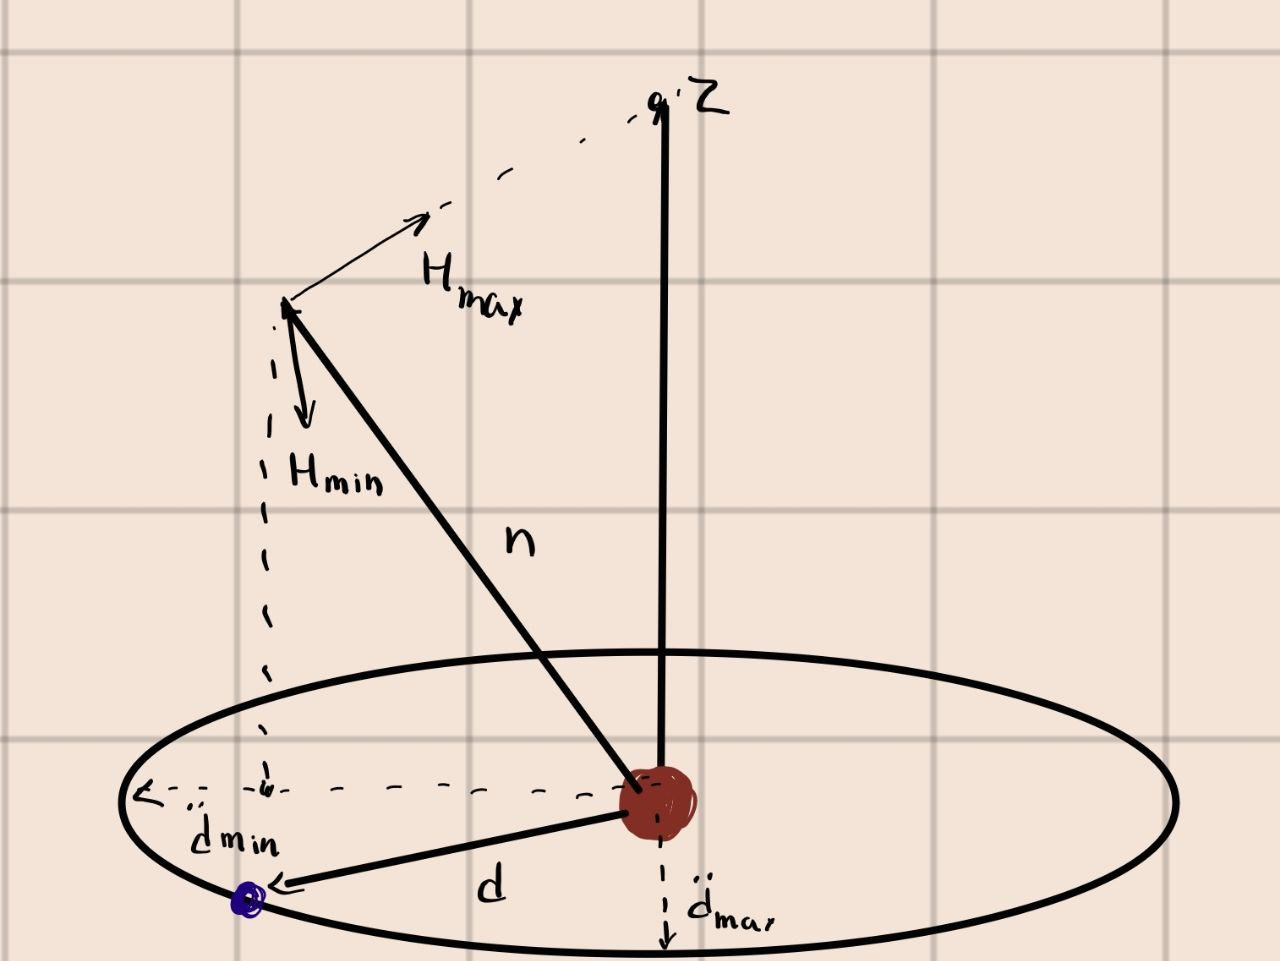
\includegraphics[trim={0 0 0 0},clip,width=1\textwidth]{sours_img/rot.jpg}
\end{figure}


